\documentclass{article}

% basics
\usepackage[margin=1in]{geometry}
\usepackage{mathptmx}

\parindent 0pt
\parskip 4pt

% section headings
\usepackage{titlesec}
% (A copy of titlesec.sty is included because there was a numbering bug in the 2016 release, which is still in wide circulation.)
\titleformat*{\section}{\bfseries\scshape\large\centering}
\titleformat*{\subsection}{\bfseries}
\titleformat*{\subsubsection}{\itshape\bfseries}

% table of contents
\usepackage[titles]{tocloft}
\renewcommand\cftsecfont{\normalfont}
\renewcommand\cftsecpagefont{\normalfont}

% figures
\usepackage{graphicx}

% tables
\usepackage{booktabs}
\setlength\heavyrulewidth{0.15em}
\cmidrulekern 0.2em
\usepackage{multirow} 
\renewcommand\multirowsetup{\centering}

% lists
\usepackage{enumitem}
\setitemize{noitemsep, topsep=-4pt, parsep=0pt, partopsep=0pt}
\setenumerate{noitemsep, topsep=0pt, parsep=0pt, partopsep=0pt}

% links
\usepackage{hyperref}
\hypersetup{colorlinks=true, linkcolor=blue, urlcolor=blue, citecolor=black}
\usepackage{url}
\def\UrlFont{\em}

% cross-refs
\usepackage[capitalize, sort&compress, nameinlink]{cleveref}
\newcommand{\crefrangeconjunction}{--}
\crefname{section}{Sect.}{Sects.}
\crefname{equation}{Eq.}{Eqs.}
\crefformat{equation}{Eq.~#2#1#3}
\crefrangeformat{equation}{Eqs.~#3#1#4--#5#2#6}
\crefmultiformat{equation}{Eqs.~#2#1#3}{--#2#1#3}{, #2#1#3}{ and~#2#1#3}

% citations
\usepackage{natbib}
\bibpunct{(}{)}{;}{a}{}{,}
\setlength{\bibsep}{4pt}
\renewcommand{\bibsection}{\subsection{References}}

% to make future picky-ness less tedious
\usepackage{xspace}
\newcommand*{\ie}{i.e.,\xspace}
\newcommand*{\eg}{e.g.,\xspace}
% \newcommand*{\ie}{i.e.\@\xspace}
% \newcommand*{\eg}{e.g.\@\xspace}
\makeatletter
\newcommand*{\etc}{%
    \@ifnextchar{.}%
        {etc}%
        {etc.\@\xspace}%
}
\makeatother

% definitions specific to this document
\newcommand{\phycomb}{PhyCoMB\xspace}
\newcommand{\Benchmark}{\textit{BenchmarkSet}\xspace}
\newcommand{\Benchmarks}{\textit{BenchmarkSet}s\xspace}
\newcommand{\Element}{\textit{Element}\xspace}
\newcommand{\Elements}{\textit{Element}s\xspace}
\newcommand{\Method}{\textit{Method}\xspace}
\newcommand{\Methods}{\textit{Method}s\xspace}
\newcommand{\Performance}{\textit{Performance}\xspace}
\newcommand{\Refset}{\textit{ReferenceSet}\xspace}
\newcommand{\Refsets}{\textit{ReferenceSet}s\xspace}
\newcommand{\Report}{\textit{Report}\xspace}
\newcommand{\Task}{\textit{Task}\xspace}
\newcommand{\Tasks}{\textit{Task}s\xspace}
\newcommand{\Trait}{\textit{Trait}\xspace}
\newcommand{\Traits}{\textit{Traits}\xspace}
\newcommand{\Tree}{\textit{Tree}\xspace}
\newcommand{\Trees}{\textit{Tree}s\xspace}

\title{Plans for the Phylogenetic Comparative Methods \\ Benchmark Database (\phycomb)}
\author{}

\begin{document}

\maketitle
\tableofcontents

\section{Introduction}

This document is intended to be a high-level description of the functionality and structure of what \phycomb will eventually look like.
Ultra-briefly:
The goal is to allow users to compare the performance of different phylogenetic methods.
There will be a web interface that allows for browsing those performance results, and for contributing new results.
Behind that will be a database of the testing datasets, methods, and results.

\section{Proposal Content}

Here is what was originally proposed to NSF/BSF.
It is still pretty much what I have in mind, but the subsequent sections provide much more detail.

\bigskip

PhyCoMB will challenge new methods in a standardized manner, revealing their strengths and weaknesses early in their lifecycle.
It will focus on testing if discrete traits affect rates of speciation and extinction, but the work will also support questions of trait evolution and lineage diversification separately.

\subsection{Community resource for benchmark tests of model performance}

A paper introducing a new phylogenetic comparative method typically includes 
essential simulations that examine its power and bias and reveal the parameter space in which it will be most beneficial.
These simulations typically follow the assumptions of the underlying model.
% Add refs to methods papers that only do this?  most of the sse papers, biogeography? traitrate? chromevol? bamm? bokma? paradis? birth-death? medusa?; hisse is a notable exception
Poor behavior, however, may arise when those assumptions are not met.
Because all empirical datasets have been shaped by processes outside the assumptions of any model, it seems self-evident that methods should routinely be tested in many situations beyond their specific focus.
Why is this not standard practice for comparative methods developers?
It is time-consuming or impossible for a single developer to craft diverse testing datasets that encompass the biological phenomena likely to `break' his/her new method.
Furthermore, there is not a culture---during development, peer review, and empirical application---of valuing and hence requiring robustness testing in this field.
Thus, phylogenetic comparative methods papers typically discuss possible artifacts but fall short of providing concrete guidance about whether a method can be reliably applied to data at hand. 
% This situation is neither ideal for learning about model behavior nor empirical systems.

We aim to break these barriers to the routine, rigorous testing of new phylogenetic comparative methods by making robustness testing more straightforward.
We will develop a suite of tests that can easily be deployed to assess the performance of a new method and compare its behavior against other methods designed for the same questions.
The product will be called \textbf{PhyCoMB: Phylogenetic Comparative Methods Benchmarking} (\cref{fig:proposal_phycomb}).
% PhyCoMB will exist as a large collection of testing datasets and metadata for download, and as a web service for identifying tests and viewing method performances.
%
Benchmark tests are standard practice in many fields, from computer hardware to bioinformatics.
For example, BAliBASE \citep[the Benchmark Alignment dataBASE;][]{thompson1999, thompson2005} has been widely adopted for assessing the performance of multiple sequence alignment algorithms. % and bahr2001
Further examples of standardized benchmark tests are Assemblethon and BUSCO for genome assembly \citep{bradnam2013, simao2015} and T.~Warnow's resources for phylogeny estimation (\url{http://www.cs.utexas.edu/~phylo/datasets}).
%
PhyCoMB's structure will mirror other benchmark suites:

$\circ$ \textit{Tasks} are specific questions within the domain of phylogenetic comparative methods.
They include tests of whether evolving traits affect rates of speciation and extinction (our focal task here), clade-specific diversification rate shifts, irreversible evolution, and discrete trait correlations.

$\circ$ \textit{Methods} are procedures designed to accomplish a task.
They consist of a model or other technique (e.g, BiSSE, sister clades), plus a statistical inference framework (e.g., AIC, model averaging, sign test).
% They consist of a model (e.g., BiSSE, BAMM) or other procedure (e.g., sister clades) plus statistical inference machinery (e.g., model comparisons with AIC, parameter value comparisons obtained with MCMC, or model averaging).

$\circ$ \textit{Elements} are collections of trees and optionally traits, all with the same properties. 
They may arise from empirical or simulated data.
A method is applied to each tree/trait item within an element.

$\circ$ \textit{Reference sets} are chosen to present particular challenges to a method, within the context of a task.
Each is a group of elements.
For example, the `power' reference set includes elements with small and large trees.
The `pseudoreplication' reference set contains trees in which traits change rarely and are accidentally associated with diversification shifts. 
The `diversification heterogeneity' reference set contains trees with complex shifts in speciation, on which neutral traits are evolved.

$\circ$ \textit{Curated benchmarks} are the heart of PhyCoMB.
The underlying database will eventually contain dozens of reference sets with many thousands of elements, but we will carefully select a subset to be the benchmark test for a task.
For example, the benchmark for trait-dependent diversification might consist of 16 elements forming a progression of increasingly challenging power tests, 24 elements with different forms of pseudoreplication, and 36 elements with different forms of diversification heterogeneity and neutral trait evolution.
Manual curation will maximize the diversity of challenges faced by a method while keeping the amount of testing manageable.
Clearly-defined benchmarks will allow the performance of different methods to be easily compared by those developing new methods and those applying them to empirical systems.

$\circ$ \textit{Annotations} will make the results obtained from PhyCoMB easier to explore and interpret.
Each element will be labelled with, e.g., the number of tips and sampling completeness, 
the type of diversification process for simulated trees,
construction methods for empirical trees,
and the model of evolution for simulated traits. 
Contributors will note the origin of the element's data (literature citation or generating script). % and explain the intent of the test.

% E: We're also going to want a set of tools for producing phycomb elements.  I've already been reusing a lot of code for simulating trees and traits in various combinations.  R package PhyCoMButils or something.

$\circ$ \textit{Reports} will allow developers to see how a new method performs relative to others, and they will allow users to understand the strengths and weaknesses of a variety of methods for a given task.

For an empiricist, PhyCoMB will provide not only structured information about methods, but also the means for directed testing.
This includes scripts for creating test data that reflect properties of real data, and for running methods on them.
It can thus enhance the impact of empirical work by aiding demonstrations of the robustness of a method for the data and question at hand.
Such improved connections between methods development and empirical use will bring greater stability and transparency to the field \citep{cooper2016}.

The first life-stage of PhyCoMB will be initiated by this proposal.
We will generate a collection of elements and benchmarks (soliciting ideas during the workshop; see Broader Impacts), and we will build a web-based interface for developers and end users.
% We in fact have already assembled a suite of 40 curated elements, and as the database grows, we will solicit further ideas as a side activity during the phylogenetics workshop (see Broader Impacts). % (used to test a new method, not described here)
% The first stage will culminate in demonstrating the value of the benchmarking approach through an extensive review of the performance of all existing methods for assessing trait-dependent diversification.
This first stage will demonstrate substantial benefits to the phylogenetics community: straightforward comparisons of old and new approaches, reproducibility of results, early warnings of methodological weaknesses, and highlights of when methods are particularly powerful and robust. %, and in general better communication about how methods for trait-dependent diversification work in practice.
%
The second stage that we envision for PhyCoMB is gradual community adoption beyond the timeframe of the proposed work.
PhyCoMB will evolve through contributions of new elements, as future work uncovers complex scenarios that challenge the assumptions of our methods.
% Elements will be contributed by anyone who has a new idea for testing, and the most valuable of these will be added to the curated benchmarks.

\begin{figure}
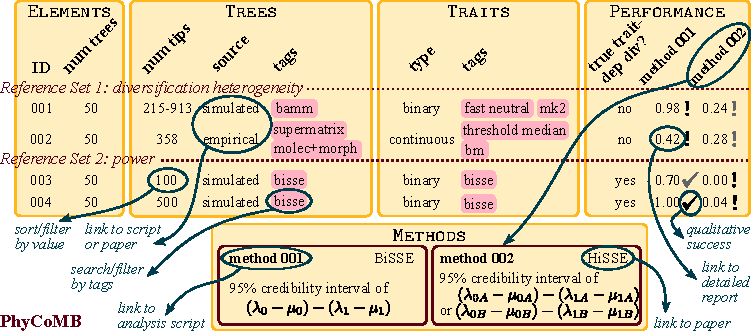
\includegraphics[width=\textwidth]{images/proposed}
\caption{
Vision for \phycomb.
The Phylogenetic Comparative Methods Benchmark database will provide test datasets and reports of method performance.
Example annotations are shown for four elements (comprising trees and traits), and interactive behavior of the web interface is noted.
Compared are two methods, which test for trait-dependent diversification by assessing the difference in estimated net diversification rates.
Performance is reported as the proportion of trees on which significant trait-dependent diversification is inferred.
Reference set 1 reveals the BiSSE-based method is prone to incorrectly associate two kinds of neutral traits with diversification rate, while the HiSSE-based method is less so.
Reference set 2 reveals that HiSSE has much lower power than BiSSE in this test.
(Note that HiSSE is much more effective under model averaging; \citealt{beaulieu2016}.)
}
\label{fig:proposal_phycomb}
\end{figure}

\bibliography{refs}
\bibliographystyle{nsf}

\subsection{Later thoughts}

This subsection wasn't part of the proposal.
But it explains some ways in which the current plan differs from what was proposed.

\bigskip

\textit{Task} needs to be defined a bit more carefully.
For example, even within the realm of state-dependent diversification, one approach/question is hypothesis testing and another approach/question is parameter estimation.
Results for those questions would be reported differently.
And even a given method on a given element could perform better on one question than the other.
Below, \textit{Task} is assumed to include this refinement.
But we could instead have a separate \textit{Question} component that intersects with \textit{Task} to specify the problem.

If we are going to include methods that co-infer the phylogeny along with answering the comparative methods question, we'd need to allow for input data to be a sequence alignment rather than a tree.
That is a potentially promising direction for methods development, but it's beyond the immediate scope of \phycomb.

\section{Users}

Different kinds of users will interact with \phycomb in different ways.
They will have different goals and permissions.
One person could be a different type of user at different times, \eg I could do some work as an Administrator, then add data as a Contributor, than look through results as a Viewer.

%--------------------------------------------------
\subsection{Viewer}
%--------------------------------------------------

Can browse \phycomb contents through the web interface.
Cannot make changes that affect anyone else.
No login required.

%--------------------------------------------------
\subsection{Contributor}
%--------------------------------------------------
\label{sec:users_contributor}

All the functionality of a Viewer.
Additionally, Contributors can see and use the parts of the web interface for uploading \Elements, \Methods, and \Performance.
Login required.

Should the newly uploaded material be immediately integrated into the database and visible to all users, or should it not be published until an Administrator approves the submission?

Contributors can't delete information, but perhaps they could flag \Elements, \etc that are no longer useful, so an Administrator could delete them.

%--------------------------------------------------
\subsection{Administrator}
%--------------------------------------------------

Can approve the uploads and suggested deletions made by Contributors.
Can also make changes to the structure (\eg which \Elements are in a \Benchmark).
Perhaps the interface will be different than what a Viewer or Contributor sees.
Login required.

\section{Workflows}

Here are some examples of how different kinds of Users might interact with \phycomb.

%--------------------------------------------------
\subsection{Explore \Performance of various \Methods for a particular \Task}
\label{sec:workflows_task}
%--------------------------------------------------

What \Methods are good or bad for my \Task of interest?

Select the desired \Task.
We will focus on ``state-dependent diversification'' with ``discrete traits,'' but eventually there might be others.
Still thinking about if we can have different possible Questions within a \Task, \eg ``Is this trait associated with diversification differences?'' versus ``Are speciation and extinction rates estimated accurately?''

Select the desired \Methods.
Choose by model/technique (\eg bisse, sister clades) and/or statistics (\eg AIC, Bayes factors).
Need a nice interface for this, but not too complicated.

Select the desired \Elements.
A few options here:
\begin{itemize}
    \item Those in the \Benchmark.
    \item Those in particular \Refsets.  Select from the list of \Refsets.
    \item Select based on attributes of \Elements, including attributes of \Trees and \Traits.  Will require a nice interface.
    \item All.  Warn how many this is.
\end{itemize}

Browse the \Performance report.
See \cref{sec:views_performance_task} for what this might look like and the types of interactivity needed.

Download the \Performance report.
See \cref{sec:downloads_report}.

%--------------------------------------------------
\subsection{Explore \Performance of a particular \Method for various \Tasks}
\label{sec:workflows_method}
%--------------------------------------------------

What \Tasks is this \Method good or bad for?

Select the desired \Method.
Default to all \Tasks, or select the desired ones.

Select the desired \Elements (see \cref{sec:workflows_task}).

Browse the \Performance report.
In this case, there will be a row for each \Task (instead of for each \Method; \cref{sec:views_performance_method}).
Need to think about if all tasks/questions can be answered with one number or symbol.

Download the \Performance report.

%--------------------------------------------------
\subsection{Contribute a new \Method}
%--------------------------------------------------

Explain why it is worthwhile---what was the purpose of creating it?
Specify what \Task it is for.
Provide basic info: what class of model/technique, what kind of statistical inference, \etc (see \cref{sec:tables_model}).
Provide a script that completely runs the \Method when provided with an \Element.
Script output should include simple summary numbers that can be provided as \Performance.
Perhaps multiple \Performance results if multiple \Tasks are addressed.
Require \Performance results for at least the \Benchmark of \Elements (see \cref{sec:workflows_performance}).

%--------------------------------------------------
\subsection{Contribute a new Element}
%--------------------------------------------------

Explain why it is worthwhile---what was the purpose of creating it?
Document so that it is completely reproducible: generating script, data source.
Include the data itself, or minimal pieces needed to generate or extract it?
Specify what it is intended for: \Task, \Refset.
Provide basic info: replicates, \Tree info, \Trait info.
Require Performance results (see \cref{sec:workflows_performance}).

%--------------------------------------------------
\subsection{Contribute new \Performance results}
\label{sec:workflow_performance}
%--------------------------------------------------

Find combinations of \Method + \Element that haven't yet be run.
Provide \Performance results.
Results could take different shapes for different \Tasks?


%--------------------------------------------------
\subsection{Deprecate a Method or Element}
%--------------------------------------------------

Don't entirely delete, but hide from most operations.
If it is superceded, could build this in to contributing the replacement.

% \section{Views}

User interfaces.

\subsection{rough}

(see \cref{sec:workflows_task})
Choose \Task.
Choose \Methods.
Choose \Elements.

%--------------------------------------------------
\subsection{\Performance report, \Task-focused}
\label{sec:views_performance_task}
%--------------------------------------------------

from \cref{sec:workflows_task}

see original proposal figure

Interactive interface:
\begin{itemize}
    \item Select tags to float \Elements to top (within a \Refset)
    \item Same, but for categories (\ie the possible values within a column)
    \item Click arrow at top of column to sort on its categories
    \item Click arrow to fold away a \Refset
    \item Click something to fold away columns?
    \item Apply a sequence of sort/filter actions.  Each refines the previous one, rather than replacing it.
    \item Clear some/all the sort/filter actions
    \item Select \Elements (rows) to hide
    \item Hide all non-floated/non-selected \Elements
\end{itemize}

Link to download CSV file.
Of entire report.
Or of just the visible part of the report (not the parts filtered/hidden).

%--------------------------------------------------
\subsection{\Performance report, \Method-focused}
\label{sec:views_performance_method}
%--------------------------------------------------

from \cref{sec:workflows_method}

Not sure how standard the task columns can be.
Need to think about if all tasks/questions can be answered with one number or symbol.

most functionality like \cref{sec:views_performance_task}

%--------------------------------------------------
\subsection{\Element}
%--------------------------------------------------

see details of a particular \Element

%--------------------------------------------------
\subsection{\Method}
%--------------------------------------------------

see details of a particular \Method

%--------------------------------------------------
\subsection{Contribute \Element}
%--------------------------------------------------

%--------------------------------------------------
\subsection{Contribute \Method}
%--------------------------------------------------
 % TODO
\section{Views [TODO]}
\section{Database Tables and Forms}
\label{sec:tables}

This section defines the fields needed for each type of information (\Element, \Tree, \etc).
Fields marked `[auto]' should be automatically populated when the contribution is saved.
All other fields should be provided by the Contributor via an input form.

I think it's realistic to settle on the set of database tables and their relationships early on.
But some of the content in the tables (columns, allowable values for some columns) will need to be adjusted as we go along.

%--------------------------------------------------
\subsection{Elements}
\label{sec:tables_element}
%--------------------------------------------------

Each \Element consists of one \Tree (\cref{sec:tables_tree}), optionally one \Trait (\cref{sec:tables_trait}), and some other information.
There should be a form for a Contributor to create a new \Element.
% The reason for \Tree and \Trait being separate entities, rather than only parts of \Element, is so they can be reused, \eg same \Tree with different \Traits makes for different \Elements.

\begin{description}
    \item[Unique ID] Arbitrary, \eg E-47295. [auto]
    \item[Date] When this was created. [auto]
    \item[Contributor] Who created this. [auto]
            Can be filled in automatically because a Contributor must be logged in to add anything new to the database (\cref{sec:users_contributor}).
    \item[Tree] Link to one \Tree.
            An existing \Tree could be selected.  (There will be too many Trees to present them all as a list.  Perhaps the Contributor could start to type the Tree's UniqueID or Name and the options could auto-complete.)
            Or, a new \Tree could be created along with this \Element (see \cref{sec:tables_tree}).
    \item[Trait] Link to one \Trait, or empty.
            (Some Tasks may not require a Trait in each Element.  But for our initial tasks, there will always be one.)
            An existing \Trait could be selected.  (Again, there will be too many Traits to present them all as a list.)
            Or, a new \Trait could be created along with this \Element (see \cref{sec:tables_trait}).
            We will need a way to check that the species names agree in a \Trait and \Tree that are part of the same \Element.
    \item[Name] A brief description of the \Element.
            Free text with a maximum of 50 characters.  Might not be unique.
    \item[Comment] Any other text the Contributor would like to provide about the \Element.
            Free text.  Formatting should be preserved.
    \item[Number of items] Positive integer.
            To avoid ambiguity, the Contributor will provide this.
            But the value should be sanity-checked against the number of items in the \Element's \Tree and \Trait.
            % Could get 50 elements via 50 trees and no traits, or via 1 tree and 50 traits, or via 50 trees and 50 traits.
    \item[Reference set] Link to one or more \Refsets (\cref{sec:tables_refset}) that this \Element will belong to.
    % \item[Benchmark] Link to \Benchmarks (\cref{sec:tables_benchmark}) that include this \Element, if any.
    \item[Correct answer] What answer should be obtained.
            The \Element will be associated with one or more \Tasks.
            (This is determined by the \Refsets selected above, which each map to \Tasks.)
            For each \Task, there is a correct answer that should be obtained from the \Element.
            Ideally, the Contributor would be presented with a small table showing each relevant \Task, with a box to provide the corresponding `Correct answer`.
            % This will be compared against the output of \Methods.
            % Each \Task will need to have a correct outcome defined.
\end{description}

% It will be common for a user to download one or more \Elements (\cref{sec:downloads_element}).

We will want to be able to find all the \Elements to which a \Tree or \Trait belongs.
From this, we can find all \Trees that use a \Trait, and all \Traits that go with a \Tree.

%--------------------------------------------------
\subsection{Trees}
\label{sec:tables_tree}
%--------------------------------------------------

It should only be possible to create a new \Tree as part of a new \Element.
Thus, the form for these \Tree fields should be part of the form for contributing an \Element.

Each \Tree object is actually a set of trees, all with the same properties.

\begin{description}
    \item[Unique ID] Arbitrary, \eg T-83247. [auto]
    \item[Date] When this was created. [auto]
    \item[Contributor] Who created this. [auto]
    \item[Number of items] The number of unique trees uploaded. [auto]
    \item[Number of tips] The number of tips per tree.  Could be a single number or a range. [auto]
    \item[Name] A brief description of the \Tree.
            Free text with a maximum of 50 characters.  Might not be unique.
    \item[Comment] Any other text the Contributor would like to provide about the \Tree.
            Free text.  Formatting should be preserved.
    \item[Source] A text file uploaded by the Contributor.
            Usually, this will be a script that generates the tree(s) or downloads them.
            If that is not possible, the file can contain notes explaining how to get the trees.
    \item[Tree files] Each individual tree is itself stored as a \href{http://evolution.genetics.washington.edu/phylip/newicktree.html}{Newick string}.
            Those strings could reside directly within the database; they can be quite long, though, which might be troublesome.
            Or the database entry could be a link to text file(s) containing the trees; this might be better because such files will frequently be downloaded by users (\cref{sec:downloads_element}).
            The Contributor will provide one text file per tree, so we should allow multiple files or one zipped file to be uploaded.
            % Or all the trees could be in a single text file, each on a new line.
    \item[Keywords] A list of options, from which the Contributor will choose one or more.
            We will want to be able to search/filter \Trees based on these values.
            The exact keywords will be determined as we go along, but a starting point is:
                `simulated',
                `empirical',
                `penalized likelihood'
    % \item [Tags] Various descriptive words.
    %     The idea with tags is that they are not necessarily alternatives (like `simulated' versus `empirical'), and there could be any number per \Tree.
    %     With use, we might realize that some tags can be converted to columns, and maybe vice versa.
    %     Tags probably involves two extra database tables:
    %     (1) columns are TagID and TagName, one row per tag;
    %     (2) columns are TreeID and TagID, one row per tag per tree.
\end{description}

%--------------------------------------------------
\subsection{Traits}
\label{sec:tables_trait}
%--------------------------------------------------

It should only be possible to create a new \Trait as part of a new \Element.
Thus, the form for these \Trait fields should be part of the form for contributing an \Element.

Each \Trait object consists of at least one trait value per species.
There could be multiple such sets in one \Trait object, \eg when simulating data so that each tree in a \Tree goes with one trait set in a \Trait.
% A \Trait isn't useful on its own---it only makes sense when associated with a \Tree.
% A \Trait will usually only correspond to one \Tree, but that's not required.
% For example, if empirical data are used to make different \Trees with different phylogenetic inference methods, we would have many \Trees and one \Trait.
All the trait sets within a \Trait have the same properties.

\begin{description}
    \item[Unique ID] Arbitrary, \eg A-57387. [auto]
    \item[Date] When this was created. [auto]
    \item[Contributor] Who created this. [auto]
    % \item[Number of trait sets] Positive integer.  Probably either 1, or one per tree.
    \item[Name] A brief description of the \Trait.
            Free text with a maximum of 50 characters.  Might not be unique.
    \item[Comment] Any other text the Contributor would like to provide about the \Trait.
            Free text.  Formatting should be preserved.
    \item[Source] A text file uploaded by the Contributor.
            Usually, this will be a script that generates the trait values or downloads them.
            It might be the same as the generating script for a corresponding \Tree.
            If there is no script, the file can contain notes explaining how to get the trait values.
    \item[Traits files] Each set of traits is simply a list of numbers, labeled by tip/species name.
            As for \Trees (\cref{sec:tables_tree}), the state info could reside directly within the database or in a linked text file (\eg CSV). % which will frequently be downloaded by users (\cref{sec:downloads_element}).
            The Contributor will provide one text file per set of traits (\ie per tree), so we should allow multiple files or one zipped file to be uploaded.
            % Or all the trait values could be in a single text file, each as a column.
    \item[Keywords] A list of options, from which the Contributor will choose one or more.
            We will want to be able to search/filter \Traits based on these values.
            The exact keywords will be determined as we go along, but a starting point is:
                `empirical',
                `simulated',
                `continuous',
                `discrete',
                `binary',
                `BM',
                `OU',
                `threshold',
                `Mk',
                `SSE',
                `neutral',
                `fast',
                `slow'
\end{description}

%--------------------------------------------------
\subsection{Reference Set}
\label{sec:tables_refset}
%--------------------------------------------------

Each \Refset is a collection of \Elements (perhaps hundreds), plus some other information.

\begin{description}
    \item[Unique ID] Arbitrary, \eg R-43853.  Auto-generated when created.
    \item[Name] A short phrase that identifies the \Refset to a human.
    \item[Description] An explanation of what this \Refset is designed to test.
    \item[Elements] Link to \Element(s) in the \Refset.  It should also be easy to obtain the total number of \Elements.
    \item[Benchmarks] Link to \Benchmark(s) that contain parts of this \Refset, if any.
    \item[Methods] Link to \Method(s) for which this \Refset is relevant.
    \item[History] Notes from Contributors who have created or changed the \Refset.  (More than one column, but I'm not sure of the best format.)
\end{description}

(I'm not sure how much linking across tables is necessary.
For example, I've included links to \Benchmark and \Method here, but perhaps those connections could be obtained merely from the \Benchmark and \Method tables themselves.)

%--------------------------------------------------
\subsection{Benchmark Set}
\label{sec:tables_benchmark}
%--------------------------------------------------

Each \Benchmark is a collection of \Elements (perhaps dozens), linked to one specific \Task, plus some other information.
These may be updated frequently, as new \Elements are added and old ones are removed.

\begin{description}
    \item[Unique ID] There won't be many of them, so we could have more meaningful names.  These could be constructed from the name of the \Task and a number (in case we want to be trying out a few benchmark sets at once).
    \item[Name] A short phrase that identifies the \Benchmark to a human.
    \item[Description] An explanation of what this \Benchmark is designed to test.
    \item[Task] Link to the \Task.
    \item[Elements] Link to \Element(s) in the \Benchmark.  It should also be easy to obtain the total number of \Elements and their \Refset membership.
    \item[Methods] Link to \Method(s) for which this \Benchmark is relevant.
    \item[Correct outcome] What answer should be obtained by an effective \Method, for a particular \Task.  This will be the same for all \Elements in the \Benchmark.
    \item[History] Notes from Contributors who have created or changed the \Benchmark.  (More than one column, but I'm not sure of the best format.)
\end{description}

%--------------------------------------------------
\subsection{Task}
\label{sec:tables_task}
%--------------------------------------------------

The top layer of organization is the \Task.
There won't be many, and perhaps only one for awhile (\ie state-dependent diversification).

Not discussed in the original proposal (\cref{sec:proposal}) is the concept of grouping tasks or questions within them.
For example, if the task is state-dependent diversification, there could be different sub-tasks for discrete-valued and continuous-valued traits.
We might also want different questions for hypothesis testing (Is my trait associated with diversification shifts?) versus parameter estimation (How much higher are speciation rates for this state?).
This latter level of detail is essential for reporting results simply (\cref{sec:tables_result}).

I think designing this layer of organization well will be quite important for \phycomb to be useful.
But we may not know the best strategy until we see how it grows.
So we'll need more discussions and probably some flexibility here.
For the moment, let's assume that \Task is defined as specifically as necessary.
This suggests using only the following fields:

\begin{description}
    \item[Unique ID] There won't be many of them, so we could have meaningful names.
    \item[Name] A short phrase that identifies the \Task to a human.
\end{description}

%--------------------------------------------------
\subsection{Methods}
\label{sec:tables_method}
%--------------------------------------------------

\cref{sec:tables_element,sec:tables_tree,sec:tables_trait,sec:tables_refset,sec:tables_benchmark,sec:tables_task} were all about the testing datasets themselves.
Now we consider the analysis methods that the tests are designed to evaluate.

\begin{description}
    \item[Unique ID] Arbitrary, \eg M-93925. [auto]
    \item[Date] When this was created. [auto]
    \item[Contributor] Who created this. [auto]
    \item[Name] A brief description of the \Method.
            Free text with a maximum of 50 characters.  Might not be unique.
    \item[Comment] Any other text the Contributor would like to provide about the \Method.
            Free text.  Formatting should be preserved.
    \item[Task] Choose from the list of existing \Tasks that this \Method is be used for.
            I'm pretty sure that each \Method can only be used for a single \Task, because the \Method can only return a single value.
            The \Task therefore determine the return value type (Boolean or numeric) of the \Method.
    \item[Analysis script] The code used to run the method.  One or more text files.
    \item[Allied methods] Note any existing \Methods that are very closely related to this one.
            There may be too many \Methods to present them all as a list.  Perhaps the Contributor could start to type the UniqueID or Name and the options could auto-complete.
            (These links will need to be updated automatically, as well.  For example, when I contribute Method 2 today I can note that it is allied with Method 1 that I created yesterday.  But then the link from Method 1 to 2 should be created automatically.)
    \item[Model-based] Choose `yes' or `no'.
    \item[Keywords] A list of options, from which the Contributor will choose one or more.
            We will want to be able to search/filter \Methods based on these values (as well as on `Model-based').
            The exact keywords will be determined as we go along, but a starting point is:
                `Akaike information criterion',
                `Bayes factor',
                `bootstrap',
                `model averaging',
                `parameter estimates',
                `posterior predictive',
                `randomization test',
                `semi-parametric',
                `sign test'
\end{description}

Methods often come in groups, and I'm not sure how to handle this.
Any thoughts or suggestions appreciated.
For example, the same basic procedure could be tweaked in a few ways (in the algorithm, or the type of stats used), and testing would reveal which was best.
Some possible approaches:
\begin{itemize}
    \item Ignore this complication.
          Each \Method is a stand-alone entity, and Contributors can just explain in the Comments if they want.
    \item Ignore this complication in the database structure, but maintain by hand a high-level summary of the available \Methods.
          Could be tough if \Methods are added frequently, though could ask Contributor for suggestions on how to update the summary accordingly.
    \item Collect enough meta-data (Columns, Tags, \etc) to generate a summary of relationships among \Methods.
          Not clear that this can usefully be done algorithmically, though.
    \item Allow one \Method to link to others.
          But then get into issues of how similar is similar enough to link (\eg `coded like' versus `inspired by').
          And then there would be lots of code reuse among scripts of different-but-related \Methods.
          [note: this is the `Allied methods' field specified above]
    \item Allow multiple analysis scripts and/or libraries of shared functions per \Method.
          Seems likely to get messy, though, especially when summarizing results.
    \item Allow one explicit level of hierarchy in \Methods.
          Contributor groups them together if they share code, but each is numbered separately and results are reported separately for each variant.
\end{itemize}

% I'm currently leaning toward the by-hand summary or the single layer of explicit hierarchy.

%--------------------------------------------------
\subsection{Results}
\label{sec:tables_result}
%--------------------------------------------------

When a \Method is run on an \Element, the output should be a clear answer to a \Task.
This is a \Result.
There will actually be a value for each Item in the \Element (\eg ten numbers if there are ten individual trees)---this is what the Contributor will provide.
We'll want \phycomb to retain this level of detail so it is available for download.
But in the \phycomb web interface, we will usually want to see a summary in which each Method-Element combination is reduced to a single value, probably the proportion of Items that yielded the correct answer (see the Outcome column in \cref{fig:ui_method_performance}).

I think the best thing here will be for a Contributor to upload a CSV file with all the information needed to compute one or more \Results.
The columns should be:
\begin{itemize}
    \item Method (its Unique ID)
    \item Element (its Unique ID)
    \item Item (1, 2, 3, \ldots)
    \item Value (TRUE/FALSE or a number)
\end{itemize}

That uploaded file will need to be checked before the contents are accepted.  Validation should include:
\begin{itemize}
    \item Each \Method exists
    \item Each \Element exists
    \item All the Items for that \Element are included
    \item The Value is of appropriate type (Boolean or numeric) for the \Method and \Task
    \item The Value does not disagree with a value that was already reported
\end{itemize}

The form for uploading \Results can be minimal: just a box for CSV file(s).

The following fields should be automatically filled in when a new \Result is created.
\begin{description}
    \item[Date] When this was created. [auto]
    \item[Contributor] Who created this. [auto]
\end{description}

We will want to be able to connect each \Element with the \Methods that run on it.
The \Results table provides this link.

One concern I have is that reducing each \Result to a single number would cause analyses to be simple-minded rather than nuanced.
On the other hand, we need to keep things simple enough that we can summarize across lots of tests and methods.
Would be good to discuss this.

We will definitely need nice ways to summarize this huge table of results for users.
These summaries are called \Reports elsewhere in this document.
But I'm not sure whether this would be done within the database structure or when generating views (\eg \cref{sec:views_report_task,sec:views_report_method}).
Some summaries we'll want:
\begin{itemize}
    \item Overall performance of a \Method on a \Refset for a \Task
    \item Overall performance of a \Method on a \Benchmark for a \Task
    \item Overall performance of a \Method at a \Task
    \item Performance of all \Methods on an \Element
    \item Performance of all \Methods on an \Refset
    \item Performance of all \Methods on an \Benchmark
\end{itemize}




%--------------------------------------------------
% "Normalization rules" for relational database structure:
% https://en.wikipedia.org/wiki/Database_normalization
% 
% 1a.  Every cell contains a single value, not a list of values.
% 1b.  No repeating group of columns (like item1, item2...).  Instead, create another table with one-to-many.
% 
% 2a.  Every non-key column is fully dependent on the primary key.
% 2b   And if the primary key is made up of several columns, every non-key column depends on the entire key.
% 
% 3a.  The non-key columns don't depend on each other.
% 3b.  They depend on the (entire) primary key (rule 2), not other non-key columns.
% 
% There are more normalization rules.  But the basic idea is to think through operations and avoid potential mistakes:
%   * Adding data:   Does it need to be added in more than one place?
%   * Changing data: Could it accidentally not be changed in all places?
%   * Deleting data: Is additional information unintentionally lost?
% 
% A normalization rule could broken to improve performance, or there can be weird situations.  But breaking a rule should be intentional, well-documented, and with extra programming logic to handle it with care.
%--------------------------------------------------

\section{Downloads}

After users view and filter the results, they may want to download information for use offline.
Each download should be a single zipped file, which contains only plain text files with a logical directory/folder structure.

%--------------------------------------------------
\subsection{Obtaining testing files}
\label{sec:downloads_element}
%--------------------------------------------------

When an \Element is downloaded, the user should receive:
\begin{itemize}
    \item Information about it (\cref{sec:tables_element}), written in an auto-generated text file.
    \item \Tree files and/or generating script and information (\cref{sec:tables_tree}).
    \item If applicable, \Trait files and/or generating script and information (\cref{sec:tables_trait}).
\end{itemize}
These files should all have sensible names.

When multiple \Elements are downloaded together, each should be in a separate directory.
If they have tree or trait files in common, could have an option to use symlinks instead of duplicating the content.
Also, a spreadsheet (CSV file, one row per \Element) should be included so it's easy to see which \Elements have which attributes (columns in \Tree, membership in \Refset, \etc).

If an entire \Refset is requested for download, each \Element within it should be in a separate directory.

If an entire \Benchmark is requested for download, each \Refset within it should be in a separate directory.

Need to decide on the file format for \Tree and \Trait.
Some options:
\begin{itemize}
    \item One Nexus file per \Element, containing all the trees and all the traits.  Uncluttered, but more annoying to parse.
    \item One file per \Tree (each line a Newick string) and one file per \Trait (CSV with one column per trait).
    \item One file per tree (many per \Tree) and one file per trait (many per \Trait), with filenames that show which belong together (\eg \texttt{t001.tre} and \texttt{s001.csv}).
\end{itemize}

% todo: link to view to access this

%--------------------------------------------------
\subsection{Obtaining methods scripts}
\label{sec:downloads_method}
%--------------------------------------------------

When a \Method is downloaded, the user should receive:
\begin{itemize}
    \item Information about it, written in an auto-generated text file.
    \item The script to run it.
\end{itemize}

When multiple \Methods are downloaded together, each should be in a separate directory.

% todo: link to view to access this

%--------------------------------------------------
\subsection{Obtaining performance reports}
\label{sec:downloads_report}
%--------------------------------------------------

The user should be able to download a CSV file that looks basically like the results table \Report (\cref{sec:views_report_task} or \cref{sec:views_report_method}).
Either the full report could be requested, or only to include those rows (\Elements) and columns that are visible after interacting with the report view.

Are additional columns needed, \eg directory names of \Elements and \Methods if they are downloaded?


\end{document}
